\documentclass[11pt]{article}
\usepackage{fullpage,amsmath, graphicx, epstopdf, tikz, amssymb, enumitem}
\usetikzlibrary{arrows}
\usepackage{amsthm}
\usepackage{todonotes}
\usepackage[linesnumbered,ruled,vlined]{algorithm2e}
\renewcommand{\baselinestretch}{1.02}
\newcommand{\Q}[1]{\medskip\item {[{\em #1 marks\/}]}\ }
\usepackage{xcolor}
\newif\ifsol
\soltrue
\newcommand{\solution}[1]{{\ifsol \color{red} {#1} \fi}}
\newcommand{\TO}{,\ldots,}

\newtheorem{claim}{Claim}

\newcommand{\down}[1]{\left\lfloor #1\right\rfloor}
\newcommand{\up}[1]{\left\lceil #1\right\rceil}
\newcommand*\Heq{\ensuremath{\overset{\kern2pt L'H}{=}}}

\begin{document}

\hfill CS 341, Spring 2020\par
\hfill Semih Salihoglu

\bigskip
\begin{center}\large\bf Assignment 7 (due Thursday, August 13th, midnight EST)
\end{center}

\noindent{\bf Instructions:}
\begin{itemize}
\item Hand in your assignment using Crowdmark. Detailed instructions are on the course website.
\item Give complete legible solutions to all questions.
\item Your answers will be marked for clarity as well as correctness.
\item For any algorithm you present, you should justify its correctness
(if it is not obvious) and analyze the complexity.
\end{itemize}

\begin{enumerate}

\Q{11} {\em Asymptotic Notation:}  

\begin{enumerate}

\Q{5} Arrange the following five functions in increasing
order of growth rate. No justifications are required. $n\log^{1000}(n)$ denotes $n \log(n) \log(n) ... \log(n)$, 
so only log(n)'s power to 1000 is taken.

$$2^{n/1000}, \text{\hspace{5pt}} n^4, \text{\hspace{5pt}} 2^{1000}n^{3.5}, \text{\hspace{5pt}} n\log^{1000}(n), \text{\hspace{5pt}} \log_{255}(1000^n)$$

$$\log_{255}(1000^n),
\text{\hspace{5pt}} n\log^{1000}(n), 
\text{\hspace{5pt}} 2^{1000}n^{3.5}, 
\text{\hspace{5pt}} n^4, 
\text{\hspace{5pt}} 2^{n/1000}
$$

\newpage
\Q {3} 
Give a simplified $\Theta$-bound (in the form $\Theta(n^k)$ for some constant $k$) for the expression
$57 n^{\sqrt{5}} + 39 \sqrt{n} \, 3^{\log_2 n}$. Briefly justify your answer.

\begin{align*}
    & \lim_{n \to \infty} \frac {57 n^{\sqrt{5}} + 39 \sqrt{n} 3^{\log_2 n}} {n^{\sqrt{5}}}\\
    = & \lim_{n \to \infty} 57 + 39 \frac {n^{\log_2 3 + 0.5}} {n^{\sqrt{5}}}\\
    = & \lim_{n \to \infty} 57 + 39 n^{\log_2 3 + 0.5 - \sqrt{5}}\\
    = & 57
\end{align*}

since $\lim_{n \to \infty} \frac {57 n^{\sqrt{5}} + 39 \sqrt{n} 3^{\log_2 n}} {n^{\sqrt{5}}} = 57$,
by theorem $57 n^{\sqrt{5}} + 39 \sqrt{n} \, 3^{\log_2 n} \in \Theta(n^{\sqrt{5}})$.

\newpage
\Q {3} Which of the following two functions has a higher growth rate? Briefly justify your answer.
\[2^{\pi \log_2 n} \quad \mbox{ or } \quad n^3 (\log_2 n)^{20}?\]

$2^{\pi \log_2 n} = (n^{\log_2 2})^\pi = n^{\pi}$\\
Hence,
\begin{align*}
    &\lim_{n \to \infty} \frac {n^{\pi}} {n^3 (\log_2 n)^{20}}\\
    = & \lim_{n \to \infty} \frac {n^{\pi - 3}} {(\log_2 n)^{20}}\\
    \Heq & \lim_{n \to \infty} \frac {(\pi - 3) n^{\pi - 4}} {20(\log_2 n)^{19} \cdot \frac {1} {\ln(2) n}}\\
    = & \lim_{n \to \infty} \frac {(\pi - 3) n^{\pi - 3}} {\frac {20} {\ln(2)} (\log_2 n)^{19}}\\
    \vdots & \\
    = & \lim_{n \to \infty} c \cdot n^{\pi - 3} \\
    = & \infty
\end{align*}
since $\lim_{n \to \infty} \frac {n^{\pi}} {n^3 (\log_2 n)^{20}} = \infty$, $2^{\pi \log_2 n}$ has a higher 
growthe rate.

\end{enumerate}

\newpage
\Q{18} {\em Short Answers}
\begin{enumerate}
\Q{2} True or False: In any connected graph G with unique edge weights, the maximum-weight edge e cannot belong to the minimum spanning tree of G. If you think the statement is true, give a short justification. Otherwise, give a counterexample.

Flase. Let $G$ be a tree, then the minimum spanning tree $T$ of $G$ is itself. Hence the maximum-weight edge is in $T$.

\newpage
\Q{2} True or False: For the all-pairs shortest paths problem, the Floyd-Warshall dynamic programming algorithm is asymptotically faster than repeated applications of Dijkstra's algorithm (from each source vertex) on sparse graphs with no negative edge weights. Briefly justify your answer. (A graph with $n$ vertices and $m$ edges is referred to as being \textit{sparse} if $m \in O(n)$.)

False. The runtime of Dijkstra's algorithm is $O(m \log n) = O(n \log n)$. The number of source vertices is 
$O(n)$. Hence the total runtime is $O(n^2 \log n)$. But the runtime of $FW$ algorithm is 
$O(n^3) > O(n^2 \log n)$.

\newpage
\Q{2} In your new company you run into a new decision problem called \textsc{Consecutive Block Minimization Problem (CBMP)} at work. You have a hard time finding a fast algorithm for it but you are able to show that there is 
a polynomial time reduction from \textsc{CBMP} to the  \textsc{Vertex Cover} problem. True or False: This proves that \textsc{CBMP} is NP-hard. Briefly justify your answer.

False. In order to prove \textsc{CBMP} is NP-hard, 
we need to prove \textsc{Vertex Cover} reduces to \textsc{CBMP}. Not the other way around.
In addition, we also need to prove \textsc{CBMP} is in $NP$.

\newpage
\Q{2} True or False: Post Correspondence Problem has an exponential time solution. Briefly justify your answer.

False. Since halting problem reduces to Post Correspondence Problem.

\newpage
\Q{2} We are given an instance $I$ of the \textsc{Stable Matching} problem with
sets  $A = \{a,b,c\}$ (e.g., interns), and $X = \{x,y,z\}$ (e.g., companies).
The instance $I$ is specified by the following preference lists, where
``$>$'' means ``prefers'':
\[
\begin{array}{l@{\hspace{1in}}l}
a : x > y > z & x : b > a > c\\
b : x > z > y & y : b > c > a\\
c : z > y > x & z : a > b > c
\end{array}
\]

Show that there is an instability in the matching
$\{ ax,bz,cy\}$. 
 
Consider the pairs $(a, x), (b ,z)$. Since $x$ prefers $b$ to $a$, and $z$ prefers $a$ to $b$, it is not stable.

\newpage
\Q{3} Show how the Gale-Shapley algorithm would execute on the instance $I$ from part (e), assuming that 
elements in $A$ propose to elements in $X$. Show all the steps in the execution of the algorithm.

\begin{enumerate}[label={\arabic*.}]
    \item add ax to the matcging 
    \item add bx to the matching, remove ax from the matching
    \item add ay to the matching
    \item add cz to the matching
    \item return matching $\{ay, bx, cz\}$
\end{enumerate}

\newpage
\Q{2} Convert the following optimization problem into its natural decision version:
\begin{quote}
{\em Input\/}: $n$ positive integers $a_1,\ldots, a_n$, a number $k$, and a positive integer $W$.\\[2pt]
{\em Output\/}: a subset $S\subseteq \{1,\ldots,n\}$ with $|S|=k$
minimizing the value $\left|\sum_{i\in S} a_i - W\right|$.  
\end{quote}

Whether there exists a subset $A$ of $\{a_1, \dots, a_n\}$ such that $|A| = k$ and $|\sum_{a \in A} a - W| = b$ 
for some value $b$.

\newpage
\Q{3} Argue briefly that if we could solve your decision problem in (g) in time
polynomial in the number of input bits, then we could also compute the 
minimum value in time polynomial in the number of input bits.

Since $\left|\sum_{i\in S} a_i - W\right|$ is bounded. So there are finite possible values of 
$\left|\sum_{i\in S} a_i - W\right|$. So we just loop throught all possible values. Intuitively, this takes 
polynomial time in the number of input bits.

\newpage
\end{enumerate}
\Q{15} {\em (Graphs)} Assume that you need to divide $n$ participants into two teams (say, team 0 and team 1). Let $N$ be the set of all participants (so $|N| = n$), and each participant $Z \in N$ can make requests of the form ``I want to be in the same team as $X$'' or ``I do not want to be in the same team as $Y$'', where $X, Y \in N$, $Z \neq X$, and $Z \neq Y$. Let the total number of such requests be $k$. The resulting teams do not have to be equal size. In an extreme case we might put all the participants into the same team. Design an $O(n+k)$ algorithm to divide the participants into two teams while satisfying all the requests, assuming that is possible. If it is impossible to satisfy the requests, then return ``Not possible". 

[Hint: convert the problem input into an appropriate graph, find the connected components of this graph. Then construct an appropriate ``meta-graph" consisting of the connected components and solve the problem on this ``meta-graph".] 

Let $Bipartition(V, E)$ be the algorithm that returns the bipartition of a graph if it is biparite and empty sets 
otherwise.

\begin{algorithm}[h]
    \caption{Divide($N, Requests$)}
    $V= N$\\
    \For{$r \in Requests$ \textbf{and} $r = \text{``i wants to be in the same team as j"}$} {
        $E[i].append(j)$\\
    }
    $C = findComponent(V, E)$\\
    \If{$|C| = 1$} {
        \Return{Not possible}
    }
    $V' = C$\\
    \For{$r \in Requests$ \textbf{and} $r = \text{``i does not want to be in the same team as j"}$} {
        Assume $i \in V(C_1)$ and $j \in V(C_2)$\\
        \If{$C_1 = C_2$}{
            \Return{Not possible}
        }
        $E'[C_1].append(C_2)$\\
    }
    $(A, B) = Bipartition(V', E')$\\
    \uIf{Bipartition does not exist, i.e. $A = B = \emptyset$} {
        \Return{Not possible}
    } \Else {
        \Return{$(A, B)$}
    }
\end{algorithm}

\textbf{Proof of Correctness:} There exists an edge $(i, j)$ if $i$ wants to be in the same team as $j$. So if 
$|C| = 1$, then all participants have to be in the same team. Hence not possible to divide the participants into 
two teams.\\
Then we contract each component into single vertex and there exists an edge $(C_1, C_2)$ if some $i$ in $C_1$ 
does not want to be in the same team as $j$ in $C_2$. In this way, the graph is biparite if and only if there 
is a way to divide participants into two teams and the bipartition is the result.

\textbf{Runtime Analysis:} Construct $G(V, E)$ takes $O(n + k)$ time. $findComponent(V, E)$ can be implemented by 
doing BFS/DFS on $G$, hence it takes $O(n + k)$ time. Construct $G'(V', E')$ takes $O(n + k)$ time. In addition, 
$Bipartition(V', E')$ can be implemented by doing BFS and coloring the nodes accodring to parity. Thus, it 
takes $O(n + k)$ time. Therefore, it is $O(n + k)$.

\newpage
\Q{14} {(\em NPC 1)} An instance $I$ of the {\sc Dominating Set} problem consists of:

\begin{itemize}
\item  an undirected graph $G_D = (V_D,E_D)$ and
\item an integer $d \leq  |V_D|$.
\end{itemize}

The output is YES iff there exists a set of $d$ vertices $U \subseteq V_D$ such that
every vertex $v \in V_D \setminus U$ is adjacent to (i.e., joined by an edge with)
at least one vertex $u \in U$.

Recall that {\sc Vertex Cover} is defined as follows: 
\begin{itemize}
\item an undirected graph $G = (V,E)$ and
\item an integer $k \leq |V|$. 
\end{itemize}
The output is YES iff there exists
a subset $S$ consisting of $k$ vertices in $V$, such that, for any edge $(u, v) \in E$, either $u \in S$ or $v \in S$ or both.

\begin{enumerate}
\Q{3} Prove that {\sc Dominating Set} is in {\bf NP}, by showing that if the answer to
an instance $I$ is YES, then using a suitable certificate/solution for $I$ and a verification algorithm,
you can verify that $I$ is indeed YES in polynomial time. It is not required to present the pseudocode, as long as your description is clear and succinct.

For every answer $U \subseteq V_D$, we can verify whether $v$ is adjacent to some vertex $u \in U$ for some 
$v \in V_D \setminus U$ in polynomial time. Since $ V_D \setminus U$ has polynomial length, we can verify 
every vertex $v \in V_D \setminus U$ is adjacent to at least one vertex $u \in U$.

\newpage
\Q{3}  Consider the following transformation (reduction) from {\sc Vertex Cover} to {\sc Dominating Set}. In your reduction, you can assume without loss of generality that the input to {\sc Vertex Cover} is a graph with at least one edge. For an instance $I = (G(V, E), k)$ of {\sc Vertex Cover}, we define an instance 
$f(I) = (G_D(V_D, E_D), d)$ of {\sc Dominating Set} as follows:
\begin{itemize}
\item $V_D = X \cup Y$ where:
\begin{itemize}
\item[] $X = \{x_v : v \in V\}$, that is for each vertex $v \in V$ there is vertex $x_v \in V_D$.
\item[] $Y = \{y_e : e \in E\}$,  that is for each edge $e$ in $E$ there is also a vertex $y_e \in V_D$.
\end{itemize}

\item $E_D = T \cup W$ where:
	\begin{itemize}
		\item[] $T = \{ (x_u, x_v): x_u,x_v \in X, x_u \neq x_v\}$, that is there is an edge in $E_D$ between every pair of vertices $x_u$ and $x_v$ in $X$.

		\item[] $W = \{(x_u, y_e), u \in V, e \in E, u \in e\}$, that is there is an edge between the vertex $x_u$ and $y_e$ in $E_D$ if $u$ is one of the vertices in edge $e$ in $E$.
	\end{itemize}

\item $d = k$.
\end{itemize}

Suppose we are given the following instance $I$ of {\sc Vertex Cover} with $k=2$:
\begin{center}
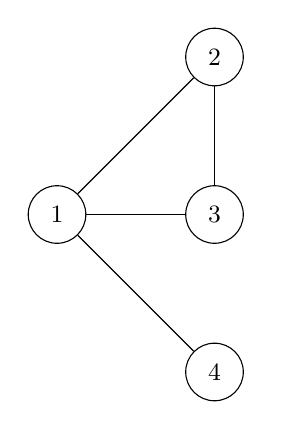
\begin{tikzpicture}
\tikzset{text width={width("10")},
	align=center,
	font=\small,auto}
\tikzset{vertex/.style = {shape=circle,draw,minimum size=1.5em}}
\tikzset{edge/.style = {-,> = latex'}}
% vertices
\node[vertex] (1) at  (-2,2) {1};
\node[vertex] (2) at  (0,4) {2};
\node[vertex] (3) at  (0,2) {3};
\node[vertex] (4) at  (0,0) {4};

%edges
\draw[edge] (1) edge node{} (2);
\draw[edge] (1) edge node{} (3);
\draw[edge] (1) edge node{} (4);
\draw[edge] (2) edge node{} (3);
\end{tikzpicture}
\end{center}

Construct the instance $f(I)$ as described above. In particular, draw the resulting graph $G_D(V_D, E_D)$.

Let edges in $E$ be 
\begin{center}
    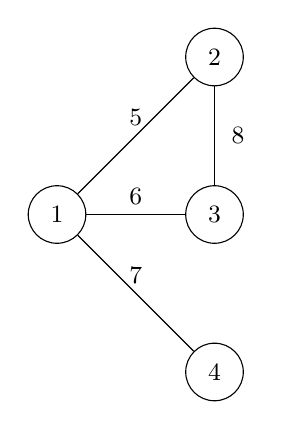
\begin{tikzpicture}
    \tikzset{text width={width("10")},
        align=center,
        font=\small,auto}
    \tikzset{vertex/.style = {shape=circle,draw,minimum size=1.5em}}
    \tikzset{edge/.style = {-,> = latex'}}
    % vertices
    \node[vertex] (1) at  (-2,2) {1};
    \node[vertex] (2) at  (0,4) {2};
    \node[vertex] (3) at  (0,2) {3};
    \node[vertex] (4) at  (0,0) {4};
    
    %edges
    \draw[edge] (1) edge node[above] {5} (2);
    \draw[edge] (1) edge node[above] {6} (3);
    \draw[edge] (1) edge node[above] {7} (4);
    \draw[edge] (2) edge node[right] {8} (3);
    \end{tikzpicture}
\end{center}

\begin{center}
    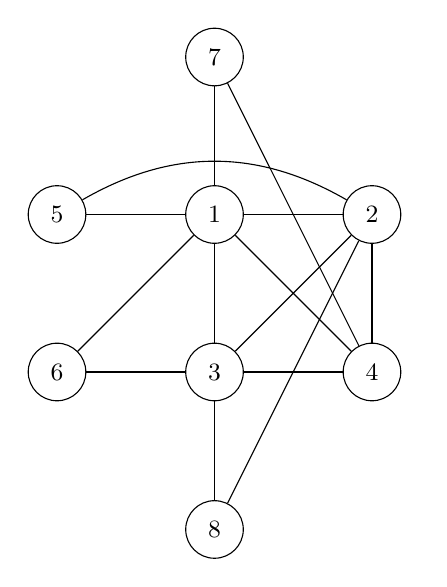
\begin{tikzpicture}
    \tikzset{text width={width("10")},
        align=center,
        font=\small,auto}
    \tikzset{vertex/.style = {shape=circle,draw,minimum size=1.5em}}
    \tikzset{edge/.style = {-,> = latex'}}
    % vertices
    \node[vertex] (1) at  (0,0) {1};
    \node[vertex] (2) at  (2,0) {2};
    \node[vertex] (3) at  (0,-2) {3};
    \node[vertex] (4) at  (2,-2) {4};
    \node[vertex] (5) at  (-2,0) {5};
    \node[vertex] (6) at  (-2,-2) {6};
    \node[vertex] (7) at  (0,2) {7};
    \node[vertex] (8) at  (0,-4) {8};
    
    %edges
    \draw[edge] (1) edge node{} (2);
    \draw[edge] (1) edge node{} (3);
    \draw[edge] (1) edge node{} (4);
    \draw[edge] (2) edge node{} (3);
    \draw[edge] (2) edge node{} (4);
    \draw[edge] (3) edge node{} (4);
    \draw[edge] (1) edge node{} (5);
    \draw[edge] (1) edge node{} (6);
    \draw[edge] (1) edge node{} (7);
    \draw[edge] (3) edge node{} (6);
    \draw[edge] (3) edge node{} (8);
    \draw[edge] (4) edge node{} (7);
    \draw[edge] (2) edge node{} (8);
    \draw[edge] (2) edge[bend right=30] node{} (5);
    \end{tikzpicture}
    \end{center}

\newpage
\Q{4} %The transformation $f$ described above can be used to prove that {\sc Dominating Set} is {\bf NP-complete}.
Prove that if $I$ is a YES-instance of  {\sc Vertex Cover}, then $f(I)$ is a YES-instance of  {\sc Dominating Set} (where $f$ is as described in part (b)).

Let $C$ be a vertex cover in $G$. For vertices $y \in Y$ in $G_D$, $y$ is adjacent to at least one vertex in $C$, 
otherwise, $C$ is not a vertex cover in $G$. For vertices $x \in X \setminus C$, since the subgraph $T$ is 
complete, $x$ is adjacent to some vertex in $C$. Hence by definition, $C$ is a dominating set in $G_D$.

\newpage
\Q{4} Prove that  $I$ is a yes-instance of  {\sc Vertex Cover} if $f(I)$ is a yes-instance of  {\sc Dominating Set}  (where $f$ is as described in part (b)).

{\bf Hint:} You may find it useful
to prove the following lemma: If $U \subseteq V_D$ is a dominating set in $G_D$, then there exists a
dominating set $U' \subseteq X$ for the graph $G_D$ such that $|U'| \leq |U|$. That is if there is a dominating set $U$ in $G_D$, then there is a dominating set $U'$ that is not larger than $U$ and only contains vertices from $X$. If you can't prove the lemma, you can still use it in your answer for partial marks.

For every vertex $v \in U$ and has an edge in $W$, $degree(v) = 2$ by construction of $G_D$. If both $v$'s neighbours $x, y$ 
are not in $U$, $U' = U \setminus \{v\} \cap \{x\}$ is also a dominating set. Since $x, v$ and $x, y$ are adjacent. 
If at least one of the neighbours are in $U$, $U' = U \setminus \{x\}$ is also a dominating set. Since $v$ is 
adjacent to $x$. We can apply the same procedure until $W \cap U' = \emptyset$. The new dominating set 
$U'$ is in $X$ and $|U'| \leq |U|$. \\
By the construction of $W$ and definition of dominating set, every edge in $G$ is adjacent to at least one 
vertex in $U'$. Hence $U'$ is a vertex  cover in $G$ with size at most $k$.

\end{enumerate}

\newpage
\Q{15} {(\em NPC 2)}
This question explores the complexity of {\sc Meeting Scheduling}.
Specifically, we want to schedule $n$ meetings
(denoted $M_1 \TO M_n$) for $\ell$ employees (denoted $E_1 \TO E_{\ell}$) 
within a period of  $K$ possible days, denoted $1\TO K$. 
For each employee $E_i$, let $S_i \subseteq \{M_1 \TO M_n\}$ denote the meetings
that $E_i$ is required to attend. 
There is no limit to the number of meetings that can be
scheduled on a given day, but we do require that no employee 
has \emph{all of their meetings on the same day}.

One way to formulate this {\sc Meeting Scheduling} problem is as follows. 
\begin{quote}
{\em Input\/}: a set $\cal M$ of $n$ elements, 
$\ell$ subsets $S_1\TO S_{\ell} \subseteq {\cal M}$,
and a positive integer $K \geq 2$.\\[2pt]
{\em Output\/}: ``yes'' if and only if there exists a
mapping $f: {\cal M}\rightarrow\{1\TO K\}$ such that
\[ \{c\in S_i: f(c)=j\} \neq S_i\] for every $i\in\{1\TO\ell\}$
and $j\in\{1\TO K\}$.
\end{quote}

Prove  that {\sc Meeting Scheduling} is NP-complete, by a reduction from
{\sc 3SAT}.  

{\em Hint\/}: It suffices to consider $K=2$.
For each clause in an input instance of {\sc 3SAT},
construct a subset involving the three literals in the clause and
\emph{one additional new element}.  You may want to construct additional 
subsets of size two, as well.

Given a solution of {\sc Meeting Scheduling}, if the answer is yes, for each $S_i$, we can verify if all the 
meetings in $S_i$ is in the same day in polynomial time. Hence we can verify all employees in polynomial time.\\
Assume {\sc 3SAT} contains $\{x_1, \dots, x_n\}$ and $m$ clauses. We add $x_{n + 1} = F$ to each clause 
$(x_i \lor x_j \lor x_k)$. The result of this new formula does not change. Since the truth value of 
$(x_i \lor x_j \lor x_k) = (x_i \lor x_j \lor x_k \lor x_{n + 1})$.Then we add clauses $(x_i \lor \neg x_i)$ 
to the formula $\phi$ if both $x_i$ and $\neg x_i$ exist in the formula. Then truth value of the new formula 
also does not change, since $(x_i \lor \neg x_i) = T$ for all values of $x_i$. Denote the new formula be $\phi'$.\\
\textbf{Claim:} There is a solution to {\sc 3SAT} if and only if there is a solution to {\sc Meeting Scheduling}\\
\begin{proof}
    $(\Rightarrow)$ Assume there is a solution to {\sc 3SAT}\\
    Apply the above procedure to $\phi$ and get $\phi'$. For clause $i$, let the variables in clause $i$ 
    be the meetings that employee $E_i$ needs to attend, $x_i = M_i$, $\neg x_i = M_{i + n + 1}$.\\
    If $x_i = T$ or $\neg x_i = T$, schedule $M_i$ or $M_{i + n + 1}$ on day one and day two otherwise.\\
    Since $\phi = T$, by th proof above, $\phi' = T$. Thus, each clause $i$ where $1 \leq i \leq n$ must have 
    a variable that has value $T$. Since $x_{n + 1} = F$, there is a variable that has value $F$. For each 
    clause $i$ where $i > n$, since it has the form of $(x_j \lor \neg x_j)$, one variable is $T$ and the other 
    is $F$. Hence, for employee $E_i$ all his/her meetings are not in the same day. \\
    $(\Leftarrow)$ Assume there is a solution to {\sc Meeting Scheduling} \\
    Assume $1 \leq i \leq n$. If $M_i$ is in day one, $x_i = T$ and $x_i = F$ otherwise. Since we guarantee that 
    $M_{i + n + 1}$ and $M_{i}$ are scheduled in diffrernt day, $x_i$ and $\neg x_i$ would have different truth 
    values. Otherwise we could have $M_i$ and $M_{i + n + 1}$ scheduled in the same day. Since all meetings of 
    a employee are not scheduled in the same day, there exists a meeting that is scheduled on day one when 
    $K = 2$. There exists a variable with truth value $T$ in every clause. Hence $\phi = T$.
\end{proof}
Thus {\sc Meeting Scheduling} is NPC.

\end{enumerate}

\end{document}

